%
% jDM08_expl_engl_galIntros.tex
%
% 
% Einleitungen f�r die Gallerien in surfer.
%
% Um aus dem pdf automatisiert ein png-Bild zu erhalten, 
% k�nnen folgende Kommandos verwendet
% werden: 
%
% pdflatex jDM08_expl_engl.tex ; pdftoppm -f 1 -l 1 -aa yes jDM08_expl_engl.pdf /tmp/jDM08_expl_engl ; convert -geometry 300x600 /tmp/jDM08_expl_engl-000001.ppm jDM08_expl_engl.png
%
%
% English version: March 2009
%
% Oliver Labs
% www.OliverLabs.net
% www.AlgebraicSurface.net
%         
%

\documentclass[sans]{amsart}

%
% Die folgenden Zeilen setzen H�he und Breite der Gallerie-Einleitungen fest:
%
\newlength{\galIntroHeight}
\newlength{\galIntroWidth}
\setlength{\galIntroHeight}{12cm}
\setlength{\galIntroWidth}{10.34cm}

%
% Die folgenden Zeilen setzen H�he und Breite des Erkl�rungs-Textes fest:
%
\newlength{\explHeight}
\newlength{\explWidth}
\setlength{\explHeight}{12cm}
\setlength{\explWidth}{6cm}

%
% Die folgenden Zeilen setzen einen (leeren, d.h.\ wei�en) 
% Rahmen von 0.1 cm um den Text:
%
\usepackage[
paperheight=\galIntroHeight
,paperwidth=\galIntroWidth
%,height=9.8cm
%,width=5.8cm
,left=0.1cm
,right=0.1cm
,bottom=0.1cm
,top=0.05cm
]{geometry}

%%%%%
% it seems to me that the papersize has to be specified here and further down, too.
%
\special{papersize=\galIntroHeight,\galIntroWidth}

%
% some latex packages we might need:
%
\usepackage{showidx}
\usepackage[latin1]{inputenc}
\usepackage[T1]{fontenc}
\usepackage{latexsym}
\usepackage{amsbsy,amscd,amsmath,amstext,amsthm}
\usepackage{amsfonts}
\usepackage{amssymb}
\usepackage{color}
\usepackage{dsfont}
\usepackage{varioref}
\usepackage{epsfig}
\usepackage{eso-pic}
\usepackage{graphicx}
\usepackage[active]{srcltx}
\usepackage{hyperref}
\usepackage[german]{babel}
\usepackage{german}
\usepackage{ifthen}
\usepackage{setspace}
\onehalfspacing

%\usepackage[scaled=0.92]{helvet}
\usepackage{multicol}
\usepackage{pstricks,pst-grad}
\usepackage{rotating}

%%%%%%%%%%%%%%%%%%%%%%%%%%%%%%%%%%%%%%%%%%%%%%
%
% Layout related stuff
%
%%%%%%%%%%%%%%%%%%%%%%%%%%%%%%%%%%%%%%%%%%%%%%

%
% for no indenting for a new paragraph:
%
\setlength{\parindent}{0pt} 
\setlength{\parskip}{1ex plus 0.5ex minus 0.2ex}

%
% don't use any roman fonts:
%
\def\rmdefault{cmss}        % no roman
\def\sfdefault{cmss}
\def\ttdefault{cmtt}
\def\itdefault{sl}
\def\sldefault{sl}
\def\bfdefault{bx}

\usepackage{sfmath} % use sans serif fonts in math mode


%
% some colors we'll use further down
%
\newrgbcolor{lightgrey}{.8 .8 .8}
\newrgbcolor{lightocher}{0.9 0.9 0.7}
\newrgbcolor{ocher}{0.7 0.7 0.5}
%\newrgbcolor{lightgrey}{.8 .8 .8}
%\newrgbcolor{lightocher}{0.9 0.9 0.65}
%\newrgbcolor{ocher}{0.7 0.7 0.35}
%\newrgbcolor{lightgrey}{.8 .8 .8}
%\newrgbcolor{lightocher}{0.8 0.8 0.8}
%\newrgbcolor{ocher}{0.7 0.7 0.7}

%
%
%
\definecolor{titleHgColor}{rgb}{0.0,0.0,0.0}
\definecolor{titleFgColor}{rgb}{0.9,0.9,0.7}
\definecolor{titleFgColorSnd}{rgb}{1.0,1.0,0.8}

\definecolor{picsHgColor}{rgb}{0.0,0.0,0.0}
\definecolor{picsFgColor}{rgb}{0.9,0.9,0.7}
\definecolor{picsFgColorSnd}{rgb}{0.95,0.95,0.75}

\definecolor{textHgColor}{rgb}{1.0,1.0,1.0}
%\definecolor{textHgColor}{rgb}{0.9,0.9,0.9}
\definecolor{textFgColor}{rgb}{0.15,0.15,0.1}
\definecolor{textFgColorSnd}{rgb}{0.4,0.4,0.2}
\definecolor{textFgColorDark}{rgb}{0.1,0.1,0.07}

%
% some commands we often use:
%

%%%%%%%%%%%%%%%%%%%%%%%%%%%%
%%%The black board font
%%%%%%%%%%%%%%%%%%%%%%%%%%%
%\newcommand{\bK}{{\bf K}}
\newcommand{\bK}{{\Bbbk}}
%\newcommand{\bK}{{\mathbb k}}
\newcommand{\AAA}{{\mathbb A}}
\newcommand{\BB}{{\mathbb B}}
\newcommand{\CC}{{\mathbb C}}
\newcommand{\DD}{{\mathbb D}}
\newcommand{\EE}{{\mathbb E}}
\newcommand{\FF}{{\mathbb F}}
\newcommand{\GG}{{\mathbb G}}
%\newcommand{\HH}{{\mathbb H}}
\newcommand{\II}{{\mathbb I}}
\newcommand{\JJ}{{\mathbb J}}
\newcommand{\KK}{{\mathbb K}}
%\newcommand{\LL}{{\mathbb L}}
\newcommand{\MM}{{\mathbb M}}
\newcommand{\NN}{{\mathbb N}}
%\newcommand{{\mathbb O}}
\newcommand{\PP}{{\mathbb P}}
\newcommand{\QQ}{{\mathbb Q}}
\newcommand{\RR}{{\mathbb R}}
\newcommand{\SSS}{{\mathbb S}}
\newcommand{\TT}{{\mathbb T}}
\newcommand{\UU}{{\mathbb U}}
\newcommand{\VV}{{\mathbb V}}
\newcommand{\WW}{{\mathbb W}}
\newcommand{\XX}{{\mathbb X}}
\newcommand{\YY}{{\mathbb Y}}
\newcommand{\ZZ}{{\mathbb Z}}


\newcommand{\dontshow}[1]{}

\newcommand{\smcdot}{{\textup{$\cdot$}}}

%%%%%%%%%%%%%%%%%%%%%%%%%%%%%%%%%%%%%%%%%%%%%%%%%%%%%%%%%%%%%%%%%%%%%%%
%
% Begin: surfer stuff
% (Some environments for the text pages for the surfer software)
%
%%%%%%%%%%%%%%%%%%%%%%%%%%%%%%%%%%%%%%%%%%%%%%%%%%%%%%%%%%%%%%%%%%%%%%%

\newenvironment{surferGalIntroPage}{%
  % start a new page, if necessary
  \newpage
 % \twocolumn
  % it seems to me that the papersize has to be specified here and further up, too
  \special{papersize=\galIntroHeight,\galIntroWidth}
  % the page background color:
  \pagecolor{textHgColor}
  % the page font color:
  \color{textFgColor}
  % no page headers or footers:
  \thispagestyle{empty}
  %%%%% 
  \begin{flushleft}}%
  {\end{flushleft}}


\newenvironment{surferPage}{%%%%% 
  % start a new page, if necessary
  \newpage
  % it seems to me that the papersize has to be specified here and further up, too
  \special{papersize=\explHeight,\explWidth}
  % the page background color:
  \pagecolor{textHgColor}
  % the page font color:
  \color{textFgColor}
  % no page headers or footers:
  \thispagestyle{empty}
  %%%%% 
  \begin{flushleft}}%
{\end{flushleft}}

\newenvironment{surferTitle}{\bf}{

}

\newenvironment{galTitle}{\bf}{

}

\newenvironment{surferText}{}{}

%%%%%%%%%%%%%%%%%%%%%%%%%%%%%%%%%%%%%%%%%%%%%%%%%%%%%%%%%%%%%%%%%%%%%%%
%
% End of: surfer stuff
%
%%%%%%%%%%%%%%%%%%%%%%%%%%%%%%%%%%%%%%%%%%%%%%%%%%%%%%%%%%%%%%%%%%%%%%%


%%%%%%%%%%%%%%%%%%%%%%%%%%%%%%%%%%%%%%%%%%%%%%%%%%%%%%%%%%%%%%%%%%%%%%%
%
% The document starts here:
%
\begin{document}
\footnotesize
% 
% Einfache Singularit�ten 
%
\begin{surferGalIntroPage}

\begin{surferTitle}Weltrekord-Fl�chen\end{surferTitle}
  % 
  \begin{surferText}
    Eine Fl�che hei�t \emph{nicht-singul�r} oder \emph{glatt}, wenn sie keine spitzen Stellen oder Selbstdurchdringungen (\emph{Singularit�ten} genannt) hat, z.B.\ eine Kugel oder ein Torus, siehe Abbildung. 
    Dies ist so gut wie immer der Fall, wenn wir die
    Fl�che zuf�llig w�hlen. 
    \begin{center}
      \vspace{-0.2cm}
      \begin{tabular}{@{}c@{}c@{}c@{\quad}c@{}c@{}c@{}c@{}}
        \begin{tabular}{@{}c@{}}
          glatt:
        \end{tabular}
        &
        \begin{tabular}{@{}c@{}}
          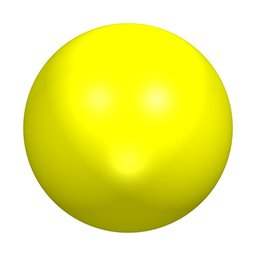
\includegraphics[width=1.1cm]{./../../common/images/kugel}
        \end{tabular}
        &
        \begin{tabular}{@{}c@{}}
          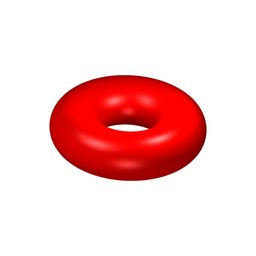
\includegraphics[width=1.1cm]{./../../common/images/torus}
        \end{tabular}
        &
        \begin{tabular}{@{}c@{}}
          viele\\
          Singularit�ten:
        \end{tabular}
        &
        \begin{tabular}{c@{}@{}}
          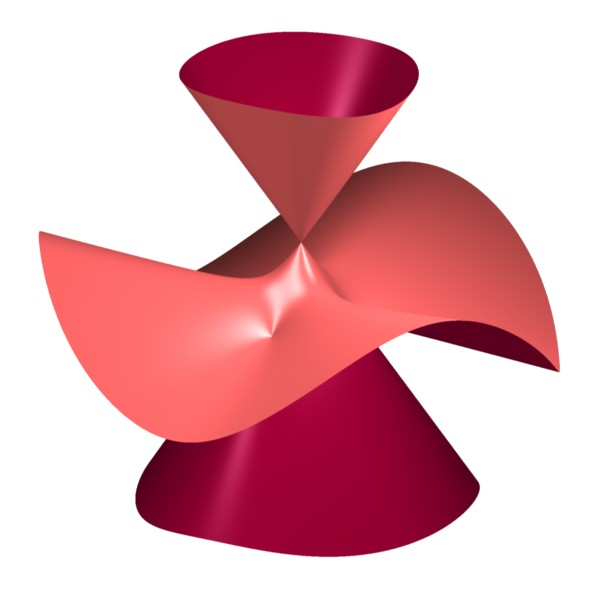
\includegraphics[width=1.1cm]{./../../common/images/cayley}
        \end{tabular}
        &
        \begin{tabular}{c@{}@{}}
          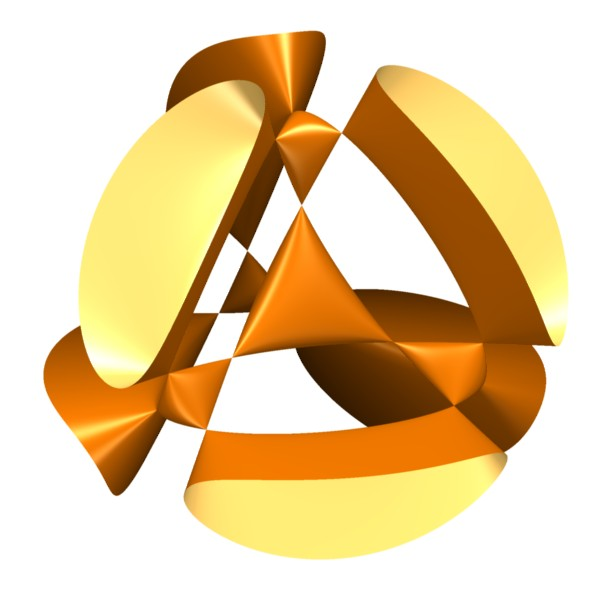
\includegraphics[width=1.1cm]{./../../common/images/kummer}
        \end{tabular}
        &
        \begin{tabular}{c@{}@{}}
          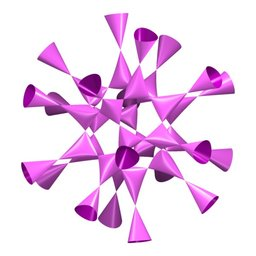
\includegraphics[width=1.1cm]{./../../common/images/barth_sextic}
        \end{tabular}
      \end{tabular}
    \end{center}
    \vspace{-0.2cm}
    Nur spezielle Fl�chen weisen Singularit�ten auf. Das macht diese Singularit�ten zu den interessantesten Punkten der Fl�che. 
    Alle Fl�chen im SURFER bestehen aus den Nullstellen von Polynomen. Das bedeutet, dass die Variablen in den Formeln nur ganzzahlige positive Exponenten haben. Den h�chsten Exponenten des Polynoms bezeichnet man auch als \emph{Grad} des Polynoms. 
    In der Mathematik lautet eine Frage in der Forschung wie viele Singularit�ten eine Fl�che mit einem bestimmten Grad haben kann. 
    Den Grad eines Polynoms bezeichnen wir mit $d$ und die Anzahl der Singularit�ten mit $\mu(d)$. Diese Zahl $\mu(d)$ ist sehr schwer zu ermitteln. F�r kleine Exponenten wie $d=1,2,3,4$ ist sie seit dem 19.\ Jahrhundert bekannt, doch f�r
    $d=5$ wurde die Zahl erst 1980 und f�r $d=6$ sogar erst 1996 herausgefunden.
    F�r ein Polynom vom Grad $7$ ist die maximale Anzahl der Singularit�ten bislang unbekannt. Es gibt jedoch schon einige Untersuchungen dazu.
    Eine endg�ltige Beantwortung der Frage f�r beliebiges $d$  liegt also noch in weiter Ferne.
    Einige bisher bekannte Werte:

    \begin{center}
      \begin{tabular}{r|cccccccc|c}
        $d$ & $1$ & $2$ & $3$ & $4$ & $5$ & $6$ & $7$ & $8$ & $d$\\
        \hline
        \hline
        \rule{0pt}{1.2em}$\mu(d)\ge$ & $0$ & $1$ & $4$ & $16$ & $31$ & $65$ &
        $99$ & $168$ & 
        $\approx \frac{5}{12}d^3$\\[0.3em]
        \hline
        \rule{0pt}{1.2em}$\mu(d)\le$ & $0$ & $1$ & $4$ & $16$ & $31$ & $65$ &
        $104$ & $174$ & $\approx \frac{4}{9}d^3$
      \end{tabular}
    \end{center}
\end{surferText}
  \end{surferGalIntroPage}
% Einfache singul�re Fl�chen
%
%
% Weltrekorde:
%
\end{document}
%
% end of the document.
%
%%%%%%%%%%%%%%%%%%%%%%%%%%%%%%%%%%%%%%%%%%%%%%%%%%%%%%%%%%%%%%%%%%%%%%%
